\section{Method of characteristics}




In previous work, we have been successful in describing birth-death dynamics of pathogenic particles inside a host cell which can rupture. In future, we wish to extend this understanding to cases with multiple host cells sharing a medium. Setting up a model with more than one host requires consideration of what happens when the first one ruptures. The shared medium suddenly gains a potentially large cohort of pathogenic particles, available for subsequent absorption by remaining hosts. We have begun to develop the analysis under the assumption of what may be called ``immediate transfer'' --- the whole pathogenic contents of a rupturing cell being relocated to the intracellular environment of another host. This is quite a hard assumption. Another, perhaps more realistic restriction might be to incorporate an ``absorption period'': following a host cell rupture, absorption events relocate the pathogenic cohort between remaining hosts. Then, only when every pathogen has been taken in, do birth death and rupture continue. 

Working towards an understanding of such ``absorption models'', we can begin by considering processes where a pathogenic cohort infiltrate only a single host cell. 

\subsection{Only absorption} 
Perhaps the most simple case for an absorption process is that of a single host cell, able to take-in pathogenic particles, but in which no subsequent dynamics take place --- without any birth, or death of pathogen within the host. 

We can introduce the variables $\xt$ \& $\yt$ to represent the number of pathogenic particles within, and outside of the host cell respectively. The same labelling will be used in later versions of the single-host model. In all cases, events will be assumed to be stochastic, happening between exponentially distributed inter-event times. This property arises from the assumption that event-rates are time-independent. It then follows that our continuous-time stochastic process, $\{(\xt, \yt) : t\in[0,\infty\}$, conforms to the memoryless Markov property.

With only absorption to consider, the model can be specified by the following probabilities --- outcome-likelihoods over an infinitesimal duration, $\Delta t$ (taken in the limit to 0).
%\begin{equation}
  % \begin{split}
  %   \pr{\Delta\xx= 1,\;\Delta\yy = -1 \;|\; \yt = j} = j \alpha \Delta t\\
 %    \pr{\Delta\xx= 0,\;\Delta\yy = 0 \;|\; \yt = j} = 1 -  j \alpha \Delta t
 %  \end{split}
%\label{probSpec1}
%\end{equation} 
\begin{align*}
     \pr{\Delta\xx= 1,\;\Delta\yy = -1 \;|\; \yt = j} &= j \alpha \Delta t,  &&\text{(absorption)}\\
     \pr{\Delta\xx= 0,\;\Delta\yy = 0 \;|\; \yt = j} &= 1 -  j \alpha \Delta t,  &&\text{(no event)}
\end{align*} 


\noindent
where $\Delta \xx = \xx_{t+\Delta t} - \xt$ (same for $\yy$). Notice the multiplication by $j$, the number of extracellular particles --- each unit subjected to the same probability, $\alpha \Delta t$, of being taken up. 

The model's initial condition will be specified: $\xx_0 = 0$, $\yy_0 = N$. A starter population of census $N$ occupying the extracellular medium. 

Defining state probabilities, $p_{i,j}(t) = \pr{\xt = i,\; \yt = j}$, we can write down the forward Kolmogorov equations: 
\begin{equation}
\label{F1}
\ddt{\p} = \alpha(j + 1) p_{i-1,j+1} - \alpha j \p.
\end{equation}

\noindent
Then, with the probability generating function defined,
\begin{equation}
\label{pgfDef}
G(x,y,t) = \sum_i\sum_j \pt x^iy^j 
\end{equation}

\noindent
$\left(=\mathbb{E}\left[x^{\xt}y^{\yt}\right]\right)$, we can go on to derive a PDE for $G(x,y,t)$ in the following way. 

Firstly, multiply each equation in (\ref{F1}) by $x^iy^j $,
\begin{equation*}
%\label{pdeDerev1}
\pddt{\p x^iy^j} = \alpha(j + 1) p_{i-1,j+1}x^iy^j - \alpha j \p x^iy^j.
\end{equation*}

\noindent
Then sum over $i$ and $j$ for non-zero $\pt$,
\begin{equation}
\label{pdeDere2}
\sum_{i = 0}^N\sum_{j=0}^N\pddt{\p x^iy^j} = \alpha\sum_{i = 1}^{N+1}\sum_{j=-1}^{N-1}(j + 1) p_{i-1,j+1}x^iy^j - \alpha \sum_{i = 0}^N\sum_{j=0}^Nj \p x^iy^j.
\end{equation}

\noindent
(Note, for any $i, j > N$, and when $i+j \neq N$, $\pt = 0$ $\forall t$. This is because pathogenic particles in this model are neither created nor destroyed.)

Rearranging (\ref{pdeDere2}), we find 
\begin{equation*}
\label{pdeDerev2}
\sum_{i = 0}^N\sum_{j=0}^N\pddt{\p x^iy^j} = \alpha\left(x\sum_{i = 0}^N\sum_{j=0}^N j p_{i,j}x^{i}y^{j-1} -  y\sum_{i = 0}^N\sum_{j=0}^Nj \p x^iy^{j-1} \right),
\end{equation*}

\noindent
which can be written in terms of the following partial derivatives,
\begin{equation*}
\label{pdeDerev2}
\sum_{i = 0}^N\sum_{j=0}^N\pddt{\p x^iy^j} = \alpha\left(x - y\right)\sum_{i = 0}^N\sum_{j=0}^N \pdd{\p x^iy^j}{y}.
\end{equation*}

\noindent
Notice, with (\ref{pgfDef}), 
\begin{equation}
\label{PDE1}
\pddt{G(x,y,t)} = \alpha\left(x - y\right) \pdd{G(x,y,t)}{y};
\end{equation}

\noindent
the chosen initial condition corresponding to $G(x,y,0) = y^N$.
 
This first-order linear initial value problem, it turns out, proves quite difficult to solve. The method of characteristics, though practicable by definition on equations of three variables, has so far lead only to mystification.

But, as it happens, we can obtain its solution via other means. 

\subsubsection*{Benefits of the independence property}
$G(x,y,t)$, as referred to above was specific to the initial condition, $\xx_0 = 0$, $\yy_0 = N$. We may further specify the probability generating function,
\begin{equation*}
G_n(x,y,t) = \sum_i\sum_j \pr{\xt = i,\;\yt=j \;|\;\xx_0 = 0,\;\yy_0=n } x^i y^j.
\end{equation*}
In such a process of just absorption, each of the $N$ pathogenic particles will get taken up by the host cell one by one. If we were to focus our attention on a single particle of this cohort, the behaviour observed would not depend on the movements of it's neighbours. Due this property of independence, our variables $\xt$ \& $\yt$ can be thought of as the sum of $N$ sub-variables, $\xt^{(k)}$ \& $\yt^{(k)}$, each pertaining only to the movements of a single pathogenic unit: 
\begin{align*}
\xt = \xt^{(1)} + \xt^{(2)} + \dots + \xt^{(n)}\\
\yt = \yt^{(1)} + \yt^{(2)} + \dots + \yt^{(n)}
\end{align*}
This observation allows us to prove that 
\begin{equation}
\label{indRelPGF}
G_n(x,y,t) = \lrb{G_1(x,y,t)}^n:
\end{equation}
\begin{align*}
G_n(x,y,t) &= \ex{x^{\sum_{k=1}^n \xt^{(k)}} y^{\sum_{k=1}^n \yt^{(k)}}}\\
&=  \ex{\prod_{k=1}^n x^{\xt^{(k)}} \prod_{k=1}^n y^{\yt^{(k)}} }\\
&=  \prod_{k=1}^n\ex{ x^{\xt^{(k)}} y^{\yt^{(k)}} }\\
&=  \prod_{k=1}^n G_1(x,y,t)\\
&= \left(G_1(x,y,t)\right)^n
\end{align*}

\noindent
Now, consider there were only one pathogenic particle to begin with; $\xx_0 = 0$, $\yy_0 = 1$. It would after some time be absorbed, and this would be the final state of the system. No other states could be reached --- quite simply: $\pt = 0$ $\forall t$ for $i+j \neq1$.\par
We can hence fully determine the state probabilities of this simple case using the forward Kolmogorov equations.
\begin{align*}
\ddt{p_{0,1}(t)} = -\alpha p_{0,1}(t) && \ddt{p_{1,0}(t)} = \alpha p_{0,1}(t) 
\end{align*}
$\implies$
\begin{align*}
p_{0,1}(t) = \ee^{-\alpha t} && p_{1,0}(t) = 1 - \ee^{-\alpha t}
\end{align*}



\begin{figure}[H]
\begin{center}
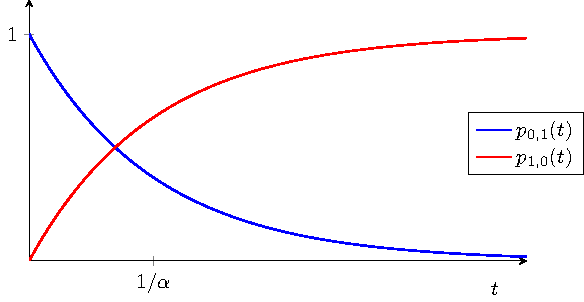
\includegraphics[width = 0.65\textwidth]{figures/IMG_ch3/abs1.pdf}
\end{center}
\end{figure}



\noindent
Given these represent the only two non-zero state probabilities of the single particle system, we can write-out the associated probability generating function as
\begin{align*}
G_1(x,y,t) &= p_{1,0}(t)x + p_{0,1}(t)y\\
    &=   \lrb{1-\ee^{-\alpha t} }x + \ee^{-\alpha t}y.
\end{align*}
Then, applying relation (\ref{indRelPGF}), we can define the probability generating function for this absorption-only system generally, for any initial state,
\begin{equation*}
G_n(x,y,t) = \lrb{ \lrb{1-\ee^{-\alpha t} }x + \ee^{-\alpha t}y}^n;
\end{equation*}

\noindent
noting that this does satisfy equation (\ref{PDE1}) along with its initial condition, 
$$G_n(x,y,0) = y^n.$$


%- forward kolmogorov equations

%- PDE for probability generating function 

%- note on difficulty in solving it

%- Solution allowed by independence assumption.

 
\subsection{Absorption-death}

In reality, when resident in a host-cell, pathogenic particles may be subject to death. \par
Setting-up a model as above, with $\xt$ \& $\yt$ representing the count of intracellular and extracellular pathogen, we can incorporate particle death with the following addition. 
\begin{align*}
     \pr{\Delta\xx= 1,\;\Delta\yy = -1 \;|\; \yt = j} &= j \alpha \Delta t,  &&\text{(absorption)}\\
      \pr{\Delta\xx= -1,\;\Delta\yy = 0 \;|\; \xt = i} &= i \mu \Delta t,  &&\text{(death)}\\
     \pr{\Delta\xx= 0,\;\Delta\yy = 0 \;|\; \yt = j, \xt=i} &= 1 -  \lrb{ j\alpha + i\mu}\Delta t,  &&\text{(no event)}
\label{probSpec1}
\end{align*} 

Form here, an analogous line of reasoning can be followed. A familiar difficulty is found on arrival at the first order linear PDE,
\begin{equation*}
\label{PDE2}
\pddt{G(x,y,t)} = \mu(1-x) \pdd{G(x,y,t)}{x}+\alpha\left(x - y\right) \pdd{G(x,y,t)}{y}.
\end{equation*}

\noindent
This point being reached from a similar derivation using the forward Kolmogorov equations:
\begin{equation*}
\label{FK1}
\ddt{\p} = \alpha(j + 1) p_{i-1,j+1} + \mu(i+1)p_{i+1,j} - (\alpha j + \mu i) \p.
\end{equation*}

\noindent
But as above, the solution can be constructed with a work-around employing the relation 
\begin{equation*}
G_n(x,y,t) = \lrb{G_1(x,y,t)}^n.
\end{equation*}

\noindent
As before, individual particles are independent from one another in their movements.\par
Without birth events, the maximum number of particles in the system is restricted to it's initial value. So, when considering the case of an isolated pathogenic unit, the probability generating function takes its form,
\begin{equation*}
G_1(x,y,t) = p_{0,0} + p_{1,0}x + p_{1,0}y.
\end{equation*}

\noindent
These state-probabilities can be determined as follows using the forward Kolmogorov equations. 
\begin{align*}
\ddt{p_{0,1}(t)} = -\alpha p_{0,1}(t) && \ddt{p_{1,0}(t)} = \alpha p_{0,1}(t) - \mu p_{1,0}(t)
\end{align*}
$\implies$
\begin{align*}
p_{0,1}(t) = \ee^{-\alpha t} && p_{1,0}(t) = \frac{\alpha}{\mu - \alpha} \Big(   \ee^{-\alpha t} - \ee^{-\mu t} \Big) && p_{0,0}(t) = 1 -p_{0,1}(t)  -p_{1,0}(t) 
\end{align*}



\begin{figure}[H]
\begin{center}
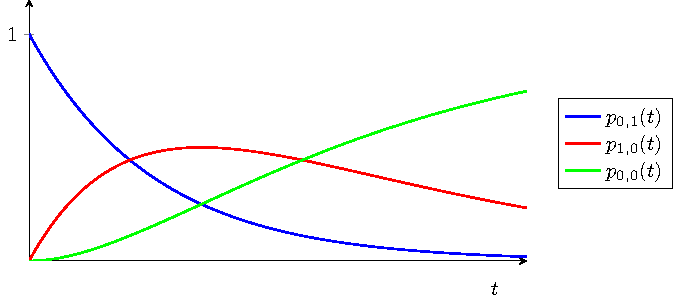
\includegraphics[width = 0.65\textwidth]{figures/IMG_ch3/abs2.pdf}
\end{center}
\caption{Caption}
\end{figure}
    

    


\noindent
Leading, as above, to the general probability generating function, $G_n(x,y,t)$, through relation (\ref{indRelPGF}):
\begin{equation*}
G_n(x,y,t) = \lrb{1-\frac{\mu}{\mu - \alpha}  \ee^{-\alpha t}  + \frac{\alpha}{\mu - \alpha} \ee^{-\mu t}  + \frac{\alpha}{\mu - \alpha} \Big(   \ee^{-\alpha t} - \ee^{-\mu t} \Big)x +  \ee^{-\alpha t} y}^n
\end{equation*}



%\begin{equation}
%G_1(x,y,t) = 1-\frac{\mu}{\mu - \alpha}  \ee^{-\alpha t}  + \frac{\alpha}{\mu - \alpha} \ee^{-\mu t}  + \frac{\alpha}{\mu - \alpha} \Big(   \ee^{-\alpha t} - \ee^{-\mu t} \Big)x +  \ee^{-\alpha t} y
%\end{equation}

\subsection{Method of characteristics (absorption-death)}

Before continuing to the case of absorption-birth-death where replication may occur within the host cell, let us revisit absorption-death from the point of its PDE for $G(x,y,t)$.  

\begin{equation}
\label{PDE2}
\pddt{G(x,y,t)} = \mu(1-x) \pdd{G(x,y,t)}{x}+\alpha\left(x - y\right) \pdd{G(x,y,t)}{y},
\end{equation}
with initial condition $G(x,y,0) = y^N$.

Since writing the above sections, I have been given advice by Benjamin Sharp on how to use the method of characteristics for 3 variate problems.\par
We begin by introducing a change of variables $(x,y,t) \to (s,r,\tau)$:
$$G(x,y,t) = G\big(x(s,r,\tau), y(s,r,\tau), t(s,r,\tau) \big) \equiv G(s,r,\tau)$$
The method works by seeking solutions on the characteristic surfaces of constant $s$ and $r$; $G(\tau)$. To do so, we must introduce an initial surface in the $s$, $r$, $\tau$ space:
\begin{align}
\label{ICpar}
x(s,r,0) = s && y(s,r,0) = r && t(s,r,0) = 0
\end{align}

With the probability generating a function of only one variable, $\tau$, we can write down the characteristic equations as ODEs. First, consider,
\begin{equation*}
\dda{G}{\tau} = \pddt{G} \dda{t}{\tau}  +  \pdd{G}{x}\dda{x}{\tau} + \pdd{G}{y}\dda{y}{\tau} .
\end{equation*}
Notice similarity with (\ref{PDE2}),
$$0  = -\pddt{G} + \mu(1-x)\pdd{G}{x} + \alpha (x-y)\pdd{G}{y}.$$
Comparing coefficients, we can write down the characteristic ODEs: 
\begin{align}
\dda{G}{\tau} &= 0\label{ch11}\\
\dda{t}{\tau} &= -1\label{ch12}\\
\dda{x}{\tau} &= \mu(1-x)\label{ch13}\\
\dda{y}{\tau} &= \alpha(x-y)\label{ch14}
\end{align}


\subsubsection*{(\ref{ch11})}
Solving the first characteristic equation,
$$\dda{G}{\tau} = 0$$
$$G = \phi(s,r)$$
$\phi$ constant on surfaces of constant $s$, and $r$.\par
With  (\ref{ICpar}), the initial condition on $G$ translates to $G(s,r,\tau=0) = r^N$, which informs us that $\phi(s,r) = r^N$. Hence,
\begin{equation}
\label{GrN}
G(s,r,\tau) = r^N.
\end{equation}



\subsubsection*{(\ref{ch12})}
$$\dda{t}{\tau} = -1$$
$$t = -\tau + c(s,r)$$
Using (\ref{ICpar}), we can fix the constant, $c(s,r) = 0$.
\begin{equation}
\label{minustau}
t = -\tau
\end{equation}


\subsubsection*{(\ref{ch13})}
$$\dda{x}{\tau} = \mu(1-x)$$
$$\vdots$$
$$1-x = c(s,r) \ee^{-\mu \tau}.$$
With initial condition, (\ref{ICpar}), $c(s,r) = 1-s$;
\begin{equation}
\label{sandxwithtau}
1-x = (1-s) \ee^{-\mu \tau}.
\end{equation}


\subsubsection*{(\ref{ch14})}

\begin{align*}
\dda{y}{\tau} &= \alpha(x-y)\\
\dda{y}{\tau} &= \alpha\left(1-(1-s) \ee^{-\mu \tau} -y\right)
\end{align*}
$$\vdots$$
$$y = 1 - \frac{\alpha}{\alpha-\mu}(1-s)\ee^{-\mu\tau} + c(s,r)\ee^{-\alpha\tau}.$$
Applying (\ref{ICpar}), $c(s,r) = r + \frac{\alpha}{\alpha-\mu}(1-s) -1$;
\begin{equation}
\label{ywithr1}
y = 1 - \frac{\alpha}{\alpha-\mu}(1-s)\ee^{-\mu\tau} + \lrb{r + \frac{\alpha}{\alpha-\mu}(1-s) -1}\ee^{-\alpha\tau}.
\end{equation}

\vspace{15pt}
\noindent
Finally, if we rearrange (\ref{ywithr1}) for $r$, also substituting $s(x,y,t)$ from (\ref{sandxwithtau}), and $\tau = -t$ from (\ref{minustau}), we find:
\begin{equation*}
r = 1-\frac{\mu}{\mu - \alpha}  \ee^{-\alpha t}  + \frac{\alpha}{\mu - \alpha} \ee^{-\mu t}  + \frac{\alpha}{\mu - \alpha} \Big(   \ee^{-\alpha t} - \ee^{-\mu t} \Big)x +  \ee^{-\alpha t} y
\end{equation*}
Then, with $G = r^N$ ((\ref{GrN})), this matches the solution obtained in the previous section, 
\begin{equation*}
G(x,y,t) = \lrb{1-\frac{\mu}{\mu - \alpha}  \ee^{-\alpha t}  + \frac{\alpha}{\mu - \alpha} \ee^{-\mu t}  + \frac{\alpha}{\mu - \alpha} \Big(   \ee^{-\alpha t} - \ee^{-\mu t} \Big)x +  \ee^{-\alpha t} y}^N.
\end{equation*}



\subsection{Absorption-birth-death}

Introducing replication for particles inside the host cell, we will see that though the independence property is still present, it no longer serves as a work-around in finding the probability generating function $G(x,y,t)$. This is because, given a single initial infections particle, with birth events, an infinite number of states can be reached. Hence $G_1(x,y,t)$ will be constituted by an infinite number of terms.\par

Thankfully, we are now also equipped to solve the PDEs for $G(x,y,t)$, and this is the approach we will take.\par

Setting up the model like in previous cases, $\xt$ \& $\yt$ represent the counts of intracellular and extracellular pathogenic particles. Birth events are added to the transition rates as follows.

\begin{align*}
     \pr{\Delta\xx= 1,\;\Delta\yy = -1 \;|\; \yt = j} &= j \alpha \Delta t,  &&\text{(absorption)}\\
     \pr{\Delta\xx= 1,\;\Delta\yy = 0 \;|\; \xt = i} &= i \beta \Delta t,  &&\text{(birth)}\\
      \pr{\Delta\xx= -1,\;\Delta\yy = 0 \;|\; \xt = i} &= i \mu \Delta t,  &&\text{(death)}\\
     \pr{\Delta\xx= 0,\;\Delta\yy = 0 \;|\; \yt = j, \xt=i} &= 1 -  \lrb{ j\alpha + i\mu + i\beta}\Delta t,  &&\text{(no event)}
\label{probSpec1}
\end{align*} 

The forward Kolmogorov equation is written as such.
\begin{equation*}
\label{FK3}
\pddt{\p } = \alpha(j + 1) p_{i-1,j+1} + \mu(i+1)p_{i+1,j}  +  \beta(i-1)p_{i-1,j}    -  (\alpha j + \mu i+\beta i) \p 
\end{equation*}

From here, again, with reasoning seen above, we can derive the associated PDE for $G(x,y,t)$.

\begin{equation}
\pddt{G} = \lrb{\mu - (\mu+ \beta)x + \beta x^2}\pdd{G}{x} + \alpha(x-y)\pdd{G}{y}
\end{equation}

To solve this by the method of characteristics, as above we re-parametrize $(x,y,t)$ to $(s,r,\tau)$, then seek solutions on characteristic surfaces of constant $s$ and $r$. Doing so brings us to the characteristic ODEs: 
\begin{align}
\dda{G}{\tau} &= 0\label{ch21}\\
\dda{t}{\tau} &= -1\label{ch22}\\
\dda{x}{\tau} &= \mu-(\mu+\beta)x + \beta x^2\label{ch23}\\
\dda{y}{\tau} &= \alpha(x-y)\label{ch24}
\end{align}
Applying the same initial conditions on $(s,r,\tau)$ as above in (\ref{ICpar}), we can solve these equations as follows.

\subsubsection*{(\ref{ch21}) \& (\ref{ch22})}
Like in the previous section the first two characteristic equations yield: 
$$G(s,r,\tau) = \phi(s,r),$$
and ultimately,
\begin{equation}
\label{gngngn}
G(s,r,\tau) = r^N.
\end{equation}
Then,
$$t = -\tau.$$   


\subsubsection*{(\ref{ch23})}
This equation looks remarkably like Jonty's equation for $S$, the survival probability. 
$$\dda{x}{\tau} = \beta\lrb{x-x_+}\lrb{x-x_-}$$
with,
$$x_{\pm} = \frac{\mu + \beta}{2\beta} \pm \sqrt{\lrb{\frac{\mu + \beta}{2\beta}}^2 - \frac{\mu}{\beta}}.$$
The main difference in its solution with Jonty's equation comes with an $s$ when fixing the constant of integration:
\begin{equation}
x(\tau) = \frac{x_+(s-x_-) - x_-(s-x_+)\ee^{\beta(x_+-x_-)\tau}}{(s-x_-) - (s-x_+)\ee^{\beta(x_+-x_-) \tau}}
\label{xabd}
\end{equation}


\subsubsection*{(\ref{ch24})}
The last characteristic equations is
$$\dda{y}{\tau} = \alpha(x-y).$$
To solve this we will need to substitute $x$ as found above, (\ref{xabd}). With an integrating factor, the equation becomes,
$$\dda{}{\tau}\lrb{\ee^{\alpha\tau} y} = \alpha \ee^{\alpha\tau} x(\tau).$$
Integrating with respect to $\tau$,
$$\ee^{\alpha\tau }y = \alpha\int \ee^{\alpha\tau} \frac{x_+(s-x_-) - x_-(s-x_+)\ee^{\beta(x_+-x_-)\tau}}{(s-x_-) - (s-x_+)\ee^{\beta(x_+-x_-) \tau}} \dd\tau.$$ 
Then splitting the numerator, 
\begin{align}
\label{bigdoubleints}
\ee^{\alpha\tau }y &=  \alpha x_+(s-x_-) \int \frac{ \ee^{\alpha \tau} } {(s-x_-) - (s-x_+)\ee^{\beta(x_+-x_-) \tau}}\dd\tau \notag \\ 
&-\alpha x_-(s-x_+)\int\frac{\ee^{\left[ \alpha + \beta(x_+-x_-) \right]\tau}}{(s-x_-) - (s-x_+)\ee^{\beta(x_+-x_-) \tau}}\dd\tau.
\end{align}

\noindent
Each of these integrals can be written in the form,
\begin{equation*}
I(\tau) = \int\frac{\ee^{h\tau}}{p+q\ee^{k\tau}}\dd\tau.
\end{equation*}
where $h$, $k$, $p$, $q$ are all constants. For example, in the first integral, $h = \alpha$, $k = \beta(x_+ - x_-)$, $p = (s-x_-)$, and $q = -(s-x_+)$. As it happens, we can solve this integral with: 
\begin{equation}
\label{hypIden}
I(\tau) = \frac{\ee^{h\tau}}{ph} {}_2F_1\lrb{1,\frac{h}{k};\frac{h}{k}+1; -\frac{q}{p}\ee^{k\tau}} + \text{const}.
\end{equation}
${}_2F_1(a,b;c;z)$ being the hypergeometric function, defined,
\begin{equation*}
{}_2F_1(a,b;c;z) =\sum^\infty_{n=0}\frac{(a)_n(b)_n}{(c)_n}\frac{z^n}{n!},
\end{equation*}
and $(p)_n$ is the (rising) Pochhammer  symbol:
$$(p)_n = \begin{cases} 1 &n=1\\
p(p+1)\cdots(p+n-1) &n>1
\end{cases}
$$
See appendix \ref{appxa} for a detailed derivation of (\ref{hypIden}).\par
Picking up again at (\ref{bigdoubleints}), the integrals are specified by (\ref{hypIden}):\\
(using $b_1 = \beta(x_+ - x_-)$ for convenience)
\begin{equation*}
\int \frac{ \ee^{\alpha \tau} } {(s-x_-) - (s-x_+)\ee^{b_1 \tau}}\dd\tau =  \frac{\ee^{\alpha\tau}}{\alpha(s-x_-)} {}_2F_1\lrb{1,\frac{\alpha}{b_1 };\frac{\alpha}{b_1 }+1; \frac{(s-x_+)}{(s-x_-)}\ee^{b_1  \tau}},
\end{equation*}
and
\begin{equation*}
\int\frac{\ee^{\left[ \alpha +b_1\right]\tau}}{(s-x_-) - (s-x_+)\ee^{b_1 \tau}}\dd\tau =   \frac{\ee^{(\alpha+b_1 )\tau}}{(\alpha+b_1 )(s-x_-)} {}_2F_1\lrb{1,\frac{\alpha + b_1 }{b_1 };\frac{\alpha + b_1 }{b_1 }+1; \frac{(s-x_+)}{(s-x_-)}\ee^{b_1  \tau}}.
\end{equation*}
Referring to these formulas as $I_1(s,r,\tau)$ and $I_2(s,r,\tau)$ respectively, and substituting into (\ref{bigdoubleints}): 
\begin{equation}
\label{eywithconst}
\ee^{\alpha\tau }y = \alpha x_+(s-x_-)I_1(s,r,\tau) - \alpha x_- (s-x_+) I_2(s,r,\tau) + \text{const}.
\end{equation}
From her, our initial condition, $y(s,r,0) = r$, fixes the constant ---
$$\text{const} = r -  \alpha x_+(s-x_-)I_1(s,r,0) + \alpha x_- (s-x_+) I_2(s,r,0).$$ 
Then, with a rearrangement of (\ref{eywithconst}), 
\begin{equation*}
r = \ee^{\alpha\tau }y - \alpha x_+(s-x_-)I_1(s,r,\tau) + \alpha x_- (s-x_+) I_2(s,r,\tau) +  \alpha x_+(s-x_-)I_1(s,r,0) - \alpha x_- (s-x_+). I_2(s,r,0)
\end{equation*}
With $I_1$, $I_2$ written explicitly,
\begin{align*}
r &= \\
 &\ee^{\alpha\tau }y\\ 
 &- \lrb{x_+ \ee^{\alpha\tau}}{}_2 F_1 \lrb{1,\frac{\alpha}{b_1 };\frac{\alpha}{b_1 }+1; \frac{(s-x_+)}{(s-x_-)}\ee^{b_1  \tau}}\\
&+\lrb{\frac{\alpha  }{\alpha + b_1}x_-\ee^{(\alpha + b_1)\tau}}{}_2F_1\lrb{1,\frac{\alpha + b_1 }{b_1 };\frac{\alpha + b_1 }{b_1 }+1; \frac{(s-x_+)}{(s-x_-)}\ee^{b_1  \tau}}\\
&+ \lrb{x_+}{}_2 F_1 \lrb{1,\frac{\alpha}{b_1 };\frac{\alpha}{b_1 }+1; \frac{(s-x_+)}{(s-x_-)}}\\
&- \lrb{\frac{\alpha  }{\alpha + b_1}x_-}{}_2F_1\lrb{1,\frac{\alpha + b_1 }{b_1 };\frac{\alpha + b_1 }{b_1 }+1; \frac{(s-x_+)}{(s-x_-)}}
\end{align*}

\noindent
From (\ref{xabd}), we have the relation,
$$\lrb{\frac{s-x_+}{s-x_-}} = \lrb{\frac{x-x_+}{x-x_-}}\ee^{b_1\tau},$$
which, applied to  the above, along with the switch, $\tau = -t$, yields 

\begin{align*}
r &= \\
 &\ee^{-\alpha t }y\\ 
 &- \lrb{x_+ \ee^{-\alpha t}}{}_2 F_1 \lrb{1,\frac{\alpha}{b_1 };\frac{\alpha}{b_1 }+1; \frac{(x-x_+)}{(x-x_-)}}\\
&+\lrb{\frac{\alpha  }{\alpha + b_1}x_-\ee^{-(\alpha + b_1)t}}{}_2F_1\lrb{1,\frac{\alpha + b_1 }{b_1 };\frac{\alpha + b_1 }{b_1 }+1; \frac{(x-x_+)}{(x-x_-)}}\\
&+ \lrb{x_+}{}_2 F_1 \lrb{1,\frac{\alpha}{b_1 };\frac{\alpha}{b_1 }+1; \frac{(x-x_+)}{(x-x_-)}\ee^{b_1  t}}\\
&- \lrb{\frac{\alpha  }{\alpha + b_1}x_-}{}_2F_1\lrb{1,\frac{\alpha + b_1 }{b_1 };\frac{\alpha + b_1 }{b_1 }+1; \frac{(x-x_+)}{(x-x_-)}\ee^{b_1  t}}
\end{align*}

\noindent
Finally, with (\ref{gngngn}),
\begin{align*}
G(x,y,t) &=\\
 &\Bigg[\ee^{-\alpha t }y\\ 
 &- \lrb{x_+ \ee^{-\alpha t}}{}_2 F_1 \lrb{1,\frac{\alpha}{b_1 };\frac{\alpha}{b_1 }+1; \frac{(x-x_+)}{(x-x_-)}}\\
&+\lrb{\frac{\alpha  }{\alpha + b_1}x_-\ee^{-(\alpha + b_1)t}}{}_2F_1\lrb{1,\frac{\alpha + b_1 }{b_1 };\frac{\alpha + b_1 }{b_1 }+1; \frac{(x-x_+)}{(x-x_-)}}\\
&+ \lrb{x_+}{}_2 F_1 \lrb{1,\frac{\alpha}{b_1 };\frac{\alpha}{b_1 }+1; \frac{(x-x_+)}{(x-x_-)}\ee^{b_1  t}}\\
&- \lrb{\frac{\alpha  }{\alpha + b_1}x_-}{}_2F_1\lrb{1,\frac{\alpha + b_1 }{b_1 };\frac{\alpha + b_1 }{b_1 }+1; \frac{(x-x_+)}{(x-x_-)}\ee^{b_1  t}}\Bigg]^N
\end{align*}


The following fact offers only some consolation from the unwieldiness of this formula.

$${}_2F_1\lrb{1,\delta;\delta+1;z} = \sum^\infty_{n=0}\frac{(1)_n(\delta)_n}{(\delta+1)_n}\frac{z^n}{n!} = \sum^\infty_{n=0}\frac{\delta}{\delta+n}{z^n}. $$

True, because along with $(1)_n = n!$, it can also be seen that 

$$\frac{(\delta)_n}{(\delta+1)n} = \frac{\delta\cancel{(\delta+1)}\cdots\cancel{(\delta + n-2)}\cancel{(\delta + n-1)}}{\cancel{(\delta+1)}\cancel{(\delta+2)}\cdots\cancel{(\delta + n-1)}(\delta + n)} = \frac{\delta}{\delta+n}.$$



\subsection*{Appendix}

\subsection{Deriving the integral result (\ref{hypIden})}\label{appxa}
To demonstrate result, 
$$\int\frac{\ee^{h\tau}}{p+q\ee^{k\tau}}\dd\tau= \frac{\ee^{h\tau}}{ph} {}_2F_1\lrb{1,\frac{h}{k};\frac{h}{k}+1; -\frac{q}{p}\ee^{k\tau}} + \text{const},$$
we will use the hypergeometric integral identity:

\begin{equation}
\label{idenHyp}
{}_2F_1(a,b;c;z) = \frac{\Gamma(c)}{\Gamma(b)\Gamma(c-b)}\int^1_0 u^{b-1}(1-u)^{c-b-1}(1-zu)^{-a} \dd u
\end{equation}
($\Gamma(x)$, being the standard gamma function). 

Taking the integral,
$$I(\tau) = \int\frac{\ee^{h\tau}}{p+q\ee^{k\tau}}\dd\tau.$$
Begin by applying the substitution, $v = \ee^{k\tau}$; with $\dd\tau = k^{-1}v^{-1} \dd v$.
\begin{align*}
I(v(\tau)) &= \frac{1}{k}\int\frac{v^{\frac{h}{k}}}{p+qv}v^{-1}\dd v\\
\notag\\
&= \frac{1}{pk}\int\frac{v^{\frac{h}{k}-1}}{1+\frac{q}{p}v}\dd v.
\end{align*}
Re-writing this as a definite integral from 0 to $v$ using a dummy variable, $s$,
$$I(v(\tau)) = \frac{1}{pk}\int^v_0\frac{s^{\frac{h}{k}-1}}{1+\frac{q}{p}s}\dd s.$$
Then, changing variables again with $s = vu$ (as $v$ is constant with regards to the definite integral, $\dd s = v\dd u$).
\begin{align}
I(v(\tau)) &= \frac{1}{pk}\int^1_0\frac{(vu)^{\frac{h}{k}-1}}{1+\frac{q}{p}vu} v \dd u\notag\\
\notag\\
&= \frac{v^{\frac{h}{k}}}{pk}\int^1_0\frac{u^{\frac{h}{k}-1}}{1+\frac{q}{p}vu}  \dd u.\label{backat}
\end{align}

\noindent
We see, this integrand lines up with that of the identity, (\ref{idenHyp});
\begin{equation*}
\int^1_0u^{\frac{h}{k}-1}(1-u)^0 \left(1-\left(-\frac{q}{p}v\right) u\right)^{-1} \dd u= \int^1_0 u^{b-1}(1-u)^{c-b-1}(1-zu)^{-a} \dd u.
\end{equation*}

\noindent
Notice, $b = \frac{h}{k}$, $c = \frac{h}{k}+1$,  $a = 1$,  and $z = -\frac{q}{p}v$. Hence,
\begin{align*}
\int^1_0\frac{u^{\frac{h}{k}-1}}{1+\frac{q}{p}vu}  \dd u &= \frac{\Gamma\left(\frac{h}{k}\right) \Gamma\lrb{1}}{\Gamma\lrb{\frac{h}{k} +1}} {}_2F_1\lrb{1,\frac{h}{k};\frac{h}{k}+1; -\frac{q}{p}v}\\
\notag\\
&= \frac{k}{h} {}_2F_1\lrb{1,\frac{h}{k};\frac{h}{k}+1; -\frac{q}{p}v},
\end{align*}
and, with (\ref{backat}),
\begin{equation*}
I(v(\tau)) = \frac{v^{\frac{h}{k}}}{ph}{}_2F_1\lrb{1,\frac{h}{k};\frac{h}{k}+1; -\frac{q}{p}v}.
\end{equation*}
Finally,
$$I(\tau) = \frac{\ee^{h\tau}}{ph}{}_2F_1\lrb{1,\frac{h}{k};\frac{h}{k}+1; -\frac{q}{p}\ee^{k\tau}}\hspace{17pt} (+ \text{const}).$$


\subsection{Extracting coefficients from the PGF -- a special case}

For a probability generating function defined not in terms of a series sum --- for example, 
\begin{equation}
\label{examplePgf}
G(t;x,y) =  \lrb{\lrb{1-\ee^{-\alpha t}}x + \ee^{-\alpha t}y}^n
\end{equation}
--- it is possible to make a conversion to its equivalent of the form,
\begin{equation}
\label{series1}
G(t;x,y) = \sum^{\infty}_{i=0}\sum^{\infty}_{j=0} p_{i,j}(t)x^iy^j.
\end{equation}
Thus extracting the time-dependent state probabilities, $p_{i,j}(t)$. It is required only that the formula $G(t;x,y)$ can be partially differentiated continuously in $x$ and $y$.\par
Here's why: A bivariate generalisation of the Maclaurin expansion can be written,
$$f(x,y)\approx Q(x,y) = \sum^{\infty}_{k=0} \lrb{\frac{1}{k!} \sum^{\infty}_{r=0}{k \choose r} \partial_x^r \partial_y^{k-r}f\bigg |_{(0,0)} x^r y^{k-r} }. $$
So, the coefficients of (\ref{series1}) can be generated via,
\begin{equation}
\label{stateProb}
p_{i,j}(t) = \lrb{i!j!}^{-1} \partial_x^i \partial_y^{j}f\big |_{(0,0)}.
\end{equation}

\subsection*{A special case}


For a probability generating function of the form,
$$G(t;x,y) = \lrb{c(t) + f(t) x + g(t) y}^n,$$
its partial derivatives in $x$ and $y$ can be obtained through
$$\partial_x^a\partial_y^b G = \lrbs{nf(t)}^a\lrbs{ng(t)}^bG.$$
With these derivatives, the state probabilities can be extracted using (\ref{stateProb}):
\begin{equation}
\label{stateProbSpec}
p_{i,j}(t) = \lrb{i!j!}^{-1} \lrbs{nf(t)}^i\lrbs{ng(t)}^jG(0,0).
\end{equation}
In this special case, $G(0,0) = (c(t))^n;$
\begin{equation}
\label{stateProbSpec2}
p_{i,j}(t) = \lrb{i!j!}^{-1} \lrbs{nf(t)}^i\lrbs{ng(t)}^j\lrbs{c(t)}^n.
\end{equation}
\subsection*{Applied to PGFs from absorption only and absorption-death }
Taking (\ref{examplePgf}), for example:
$$p_{i,j}(t) = \frac{n^{i+j}}{\lrb{i!j!}} \lrbs{1-\ee^{-\alpha t}}^i\lrbs{\ee^{-\alpha t}}^j.$$
The same can be done for 
$$G(t;x,y) = \lrb{1-\frac{\mu}{\mu - \alpha}  \ee^{-\alpha t}  + \frac{\alpha}{\mu - \alpha} \ee^{-\mu t}  + \frac{\alpha}{\mu - \alpha} \Big(   \ee^{-\alpha t} - \ee^{-\mu t} \Big)x +  \ee^{-\alpha t} y}^n$$
from the absorption-death case:
$$p_{i,j}(t) = \frac{n^{i+j}}{\lrb{i!j!}} \lrbs{\frac{\alpha}{\mu - \alpha} \Big(   \ee^{-\alpha t} - \ee^{-\mu t} \Big)}^i\lrbs{\ee^{-\alpha t}}^j\lrbs{1-\frac{\mu}{\mu - \alpha}  \ee^{-\alpha t} + \frac{\alpha}{\mu - \alpha} \ee^{-\mu t}}^n.$$
